\chapter{Fundamentals and related work}

\section{Software-Defined Networking}

The origin of Software-Defined Networking (SDN) began already in 1995, however the first use cases were only developed in 2001 and the promotion of SDN only began with the foundation of the non-profit industry consortium Open Networking Foundation (ONF) in 2011. % % https://en.wikipedia.org/wiki/Software-defined_networking % %
The ONF is dedicated to push and adapt open standards like the OpenFlow into the industry.
In this following section a brief overview of the SDN architecture and concepts, including the OpenFlow protocol is given.

\subsection{Motivation}

Today's internet is part of the modern society, be it for private users, enterprises or vital infrastructure services. Networks are required to evolve in order to address the challenges that are entailed with new applications, services and a growing number of end-users.

With a more detailed view on the challenges of current networks one comes to see the following limitations:

% % ONF White Paper (pdf): SDN - The new norm for networks % % 
\begin{itemize}
\item \textbf{Inability to scale}: With the expansion of data centers, networks must grow too. Configuring and managing these additional network devices comes at a high administrative effort. With the virtualization of data centers network traffic patterns becomes more and more dynamic and unpredictable. With multi-tenancy a further complication is introduced, because different end-users and services need different network performance and might require traffic steering. Such scaling and network management cannot be done with a manual configuration of the underlying infrastructure.
\item \textbf{Complexity}: In the past decades new networking protocols have been adapted by the industry. To add or move any device, multiple existing switches, routes, firewalls must be touched in order to manage protocol-based mechanisms on a device-level. With the virtualization of servers the amount of interfaces that need network connectivity and the distribution of applications over a number of virtual machines (VMs) are another demand that the current fairly static networks cannot dynamically adapt to.
\item \textbf{Inconsistent policies}: For IT to apply a network- or data center-wide policy a lot of devices and mechanisms may need to be reconfigured. Virtual Machines are created and rebuilt within no time, but if for example access or security needs to be updated, the benefits of this dynamic are subverted(?).
\item \textbf{Vendor dependence}: Standards are needed to match the requirements of the markets with the capabilities of networks and enable network operators to customize the network to specific environments.
\end{itemize}

Traditionally decisions about traffic flowing through the network are made directly by each network device, because the control logic and forwarding hardware are tightly coupled.

\subsubsection{Classical switches \& routers}

Packet forwarding (data plane) and routing decisions (control plane) in classical switching and routing are both within one device. In figure .. the main components that are depicted have the following functions:
\begin{enumerate}
\item The \textbf{forwarding path} typically handles data path operations for each packet. It generally consists of Application-Specific Integrated Circuits (ASIC), network-processors or general-purpose processors that forwards frames and packets at wire speed (line-rate). Their lookup functions can be further increased with memory resources like Content Addressable Memory (CAM) or Ternary Content Addressable Memory (TCAM) to contain the forwarding information.
\item The elements in the \textbf{control plane} are based on general-purpose processors that provide services like routing and signaling protocols, including ARP, MAC Learning and forwarding tables.
\end{enumerate}

\begin{figure}[hp]
\centering

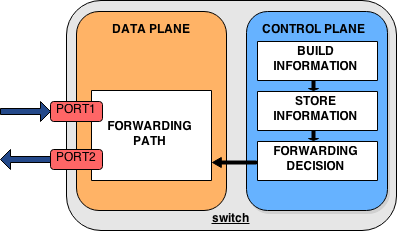
\includegraphics[width=0.5\textwidth]{images/fundamentals/switch_components}

\caption{Figure... "Classical" switch components}
\end{figure}

A switch consists of multiple ports for incoming and outgoing data. Internal forwarding tables classify the packets and forward them to one or many specific ports. It does so by collecting MAC addresses and storing their corresponding port in specific tables. Layer 2 switches also support the segregation into virtual LANs (VLAN), which enables the network operator to logically isolate networks that share a single switch.

Routers forward packets on the Network layer (Layer 3) and routing-decisions are made based on IP addresses. They contain a routing table where paths to neighbour networks are stored, so that packets can be forwarded to their destination IP address. Other features that can be configured with routers are Quality of Service (QoS), Network Address Translation (NAT) and packet filtering.

The main differences between the classical architecture and SDN will be further described in the coming sections.

\subsection{Software-Defined Networking concept}

%% https://www.opennetworking.org/sdn-resources/sdn-definition % %

SDN represents a new dynamic, manageable, cost-effective and adaptable architecture that is built to serve the dynamic infrastructures that are needed as a backbone for today's data centers. Opposed to the traditional approach, network control and forwarding functions are decoupled and thus can be programmed and divided into different applications and network services.
The work of the Open Networking Foundation laid out the OpenFlow protocol as the base for modern SDN solutions.

\subsection{SDN architecture}

SDN separates the architecture into three distinct layers that communicate with each other through different APIs. In figure .. this separation is shown.

\begin{itemize}
\item \textbf{Infrastructure Layer:} here all switching elements that are capable of the OpenFlow Protocol provide forwarding mechanisms on different Network Layers.
\item \textbf{Control Layer:} 
\item \textbf{Application Layer:} 


\end{itemize}

\begin{figure}[hp]
\centering

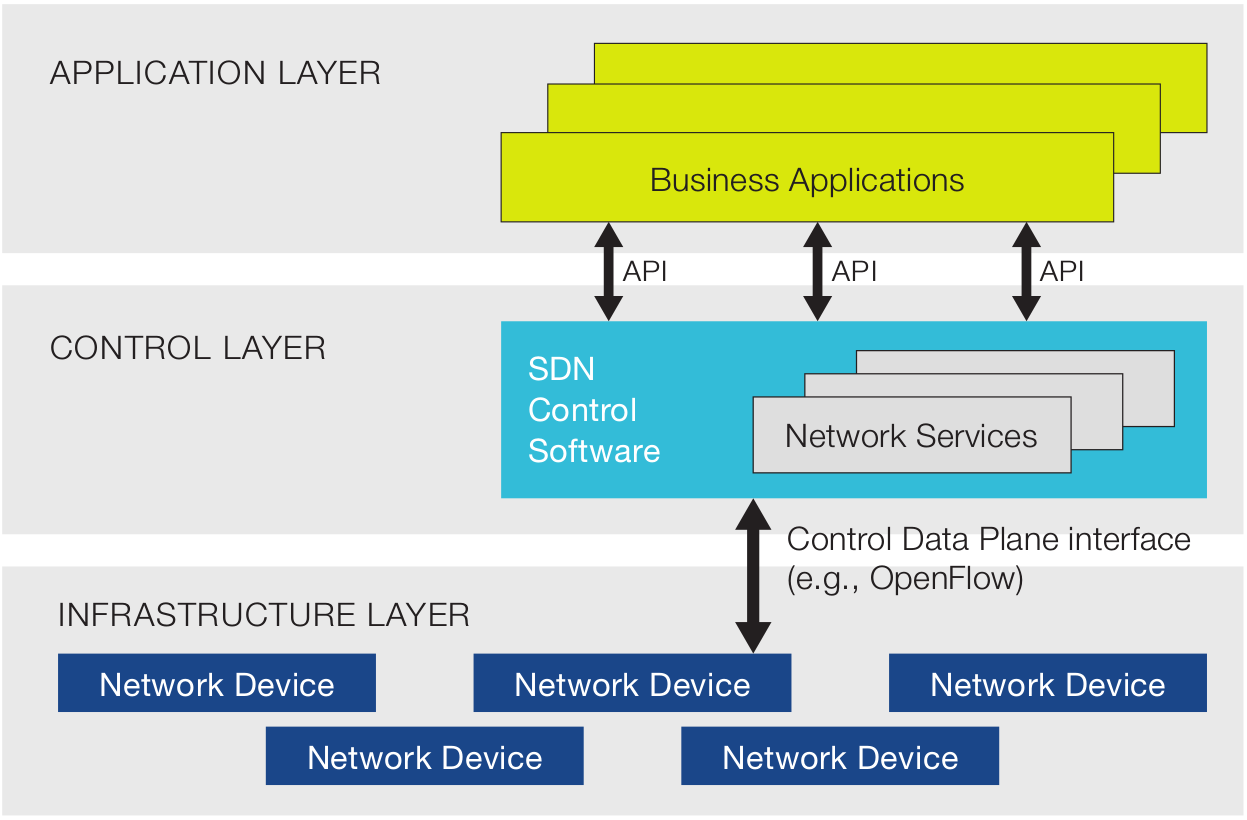
\includegraphics[width=0.7\textwidth]{images/fundamentals/sdn_logical_architecture}

\caption{Figure... Software-Defined Network architecture}
\end{figure}


\subsection{OpenFlow Controller}

\subsection{OpenFlow Switch}

\subsection{OpenFlow Software Switch}

OpenVSwitch

\section{Cloud computing infrastructures}

\subsection{OpenStack}

\subsection{Devstack}

\subsection{OpenStack Nova}

\subsection{OpenStack Heat}

\subsection{OpenStack Neutron}


\section{Conclusion}